\documentclass[12pt]{article}

\usepackage{sbc-template}
\usepackage[utf8]{inputenc}
\usepackage{graphicx,url}
\usepackage{indentfirst}
\usepackage[portuges]{babel}
\usepackage{enumitem}
\usepackage{xcolor}
\usepackage{blindtext}

\sloppy
%---------------------CAPA DO ARTIGO
\title{Mineração de Dados Educacionais para Classificação de Alunos na Universidade do Estado do Amazonas}

\author{Gabriel Alexander Teixeira, Luiz Carlos Glomyer, Abraão B. Brandão}

\address{Engenharia de Computação -- Universidade do Estado do Amazonas (UEA)
\\
\email{gaflt.eng17@uea.edu.br, glomyerjunior@hotmail.com,abraaobritof10@gmail.com}
  \\Escola Superior de Tecnologia - EST \\Endereço: Av. Darcy Vargas, 1200 - Parque Dez,\\ Manaus - AM, 69050-020
}
%------------------- FIM DA CAPA & BEGIN{DOCUMENT} = COMEÇO DO DOCUMENTO

\begin{document} 

\maketitle %Comando de Máscara de Capa

%-------------------------INICIO DO RESUMO
\begin{resumo} 
  Este artigo tem como finalidade a aplicação dos conceitos de Ciência de Dados e Mineração de Dados Educacionais para a identificação de possíveis reprovações ou desistências referentes aos alunos do campus da Universidade do Estado do Amazonas - UEA. Utilizando os conceitos de sistemas de classificação, o objetivo é demonstrar como os algoritmos de classificação podem ser utilizados para identificar alunos com problemas no aprendizado e melhorar a forma de aprendizagem dos mesmos através da supervisão de suas notas. Para a criação da proposta foram utilizados os datasets fornecidos pelo professor da disciplina e como algoritmo-base o algoritmo de Árvores de Decisão J48.
\end{resumo}
%---------------------FIM DO RESUMO
%------------------TÓPICO 1
\section{Introdução e apresentação dos softwares a serem utilizados}

A universidade é uma parte fundamentalmente importante para a vida das pessoas como um todo. Porém, algo curioso acontece quase sempre nas instituições públicas: as altas taxas de reprovação. Isto está vinculado a vários fatores sociais, como a falta de uma base sólida de conhecimentos, a adequação do aluno ao ritmo de estudos de sua antiga instituição, a falta de um lugar próprio para estudos, a falta de infraestrutura de sua universidade, dentre outros motivos. Todos estes fatores influenciam negativamente a vida acadêmica dos discentes.


Neste projeto usamos os seguintes softwares:

\begin{description}[font=$\bullet$~\normalfont\scshape\color{black!50!black}]

\item[weka] O Weka (Waikato Environment for Knowledge Analysis) é um software que agrega vários algoritmos dedicados ao estudo de aprendizagem de máquina. Ele faz uma análise computacional e estatísticas dos dados fornecidos, recorrendo a diversas técnicas de reconhecimento de padrões para, a partir daí, fazer a classificação ou regressão dos dados.
\\
\item[excel] Vindo da suíte Microsoft Office, o Excel é um editor de planilhas que possui ferramentas de cálculo e plotagem de gráficos. Ele desempenhou um papel fundamental na organização e na pré-análise dos dados fornecidos por meio de suas inúmeras funcionalidades e interface intuitiva.
\\
\item[java] Usamos a linguagem de programação Java para desenvolver a nossa aplicação, utilizando bibliotecas de machine learning e a API Java Swing para a interface gráfica.

\end{description}

%------------------TÓPICO 2
\section{Mineração de dados educacionais} 
A mineração de dados é o processo de analisar enormes quantidades de dados para detectar padrões entre variáveis, detectando asssim novos subconjuntos de dados. É, sobretudo, um campo derivado do Aprendizado de Máquina (Machine Learning), que por sua vez deriva do tópico Inteligência Artificial.

As correlações entre os dados que podem ser descobertas são:

\begin{description}[font=$\bullet$~\normalfont\scshape\color{black!50!black}]

\item[associações]  São ocorrências ligadas a um único evento. Por exemplo: um estudo de modelos de compra em supermercados pode revelar que, na compra de salgadinhos de milho, compra-se também um refrigerante tipo cola em 65\% das vezes: mas, quando há uma promoção, o refrigerante é comprado em 85\% das vezes.Com essas informações, os gerentes podem tomar decisões mais acertadas pois aprenderam a respeito da rentabilidade de uma promoção
\\
\item[sequências]  Na sequência os eventos estão ligados ao longo do tempo. Pode-se descobrir, por exemplo, que quando se compra uma casa, em 65\% as vezes se adquire uma nova geladeira no período de duas semanas; e que em 45\% das vezes, um fogão também é comprado um mês após a compra da residência.
\\
\item[classificação]Reconhece modelos que descrevem o grupo ao qual o item pertence por meio do exame dos itens já classificados e pela inferência de um conjunto de regras. Exemplo: empresas de operadoras de cartões de crédito e companhias telefônicas preocupam-se com a perda de clientes regulares, a classificação pode ajudar a descobrir as características de clientes que provavelmente virão abandona-las e oferecer um modelo para ajudar os gerentes a prever quem são, de modo que se elabore antecipadamente campanhas especiais para reter esses clientes.
\\
\item[aglomeração] Também chamado de clustering, funciona de maneira semelhante a classificação quando ainda não foram definidos grupos. Uma ferramenta de data mining descobrirá diferentes agrupamentos dentro da massa de dados. Por exemplo ao encontrar grupos de afinidades para cartões bancários ou ao dividir o banco de dados em categorias de clientes com base na demografia e em investimentos pessoais.
\\
\item[prognóstico]  Embora todas essas aplicações envolvam previsões, os prognósticos as utilizam de modo diferente. Partem de uma série de valores existentes para prever quais serão os outros valores. Por exemplo um prognóstico pode descobrir padrões nos dados que ajudam os gerentes a estimar o valor futuro de variáveis com números de vendas.

\end{description}

A mineração de dados educacionais é a área de pesquisa que tem como base a coleta, o estudo, e a aplicação de dados provenientes de ambientes educacionais. \cite{Minera:01}\cite{Lucas:17} O intuito deste estudo é encontrar e compreender os fatores que possam influenciar o aprendizado de um aluno. Fatores como a causa-raiz da evasão escolar e das reprovações são estudados com minúcia, a fim de que se possa sanar estes recorrentes problemas no escopo do ensino público. Com o auxílio de dados, poderíamos classificar o perfil de estudantes com rendimento baixo e logo após fazer previsões para identificar possíveis alunos em risco de reprovação.

Utilizamos esta abordagem com o dataset que nos foi fornecido.

%------------------TÓPICO 3
\section{Dataset: Lyceum}
Foram disponibilizados dois datasets, o dataset que contém os dados dos alunos da Universidade do Estado do Amazonas (UEA) durante o período de 2013 a 2014, e o dataset referente ao período de 2015 a 2018. O dataset possui, no total, 15 colunas: o código do aluno, o município de nascimento, a data de nascimento do aluno, o código referente ao curso, o nome do curso em si, o tipo de ingresso do aluno (Vestibular, Sistema de Ingresso Seriado), o ano de ingresso, a unidade física em que reside o aluno, a série (período), o código referente à disciplina, o nome em si da disciplina, a nota final, a situação do aluno (se foi aprovado ou se foi reprovado), a percentagem de faltas e as faltas em si.

O dataset de 2013 possui mais de 57.000 registros, enquanto o de 2015 possui mais de 60.000. Apesar de possuirmos uma enorme quantidade de dados, muitos deles não nos são úteis. Por isso, os dados analisados por nós sofreram uma leve limpeza a fim de que essa "sujeira" não afete o resultado final de nossa análise. Por exemplo, as colunas "Faltas" e "Percentual de Presença" se referem ao mesmo conceito, logo apenas uma das duas deveria ser levada em consideração. Outro tipo de registro que poderia afetar nosso resultado final são aqueles dos alunos com a matrícula trancada ou cancelada, ou seja, não possuem um índice de faltas e de notas. 

Após essa filtragem, removemos cerca de 5.000 registros em cada dataset. Essas informações, após a nossa filtragem, foram capazes de nos informar os padrões ocultos que estão contidos nos dados, como o porquê de determinada disciplina sempre ter um número tão alto de reprovações, quais são as disciplinas em que os alunos mais tem faltas.

%------------------TÓPICO 4
\section{Algoritmo ZeroR}

O algoritmo ZeroR toma o valor que mais se repete dentro de um conjunto e divide esse valor pela quantidade de registros, logo após ele classifica todos os outros elementos do conjunto como sendo este valor que mais se repete \cite{ZeroR:67}. É chamado de algoritmo de linha base, ou seja, é o algoritmo mais simples de classificação, sendo ele recomendável para que seja usado primeiramente antes de testar outros algoritmos. Se, ao testar outro algoritmo, a porcentagem de acertos deste for menor do que a da linha-base (porcentagem de acertos do ZeroR), significa que o algoritmo é ineficiente para o problema apresentado e que algum outro deve ser utilizado em seu lugar.

Usando este algoritmo superficialmente, conseguimos resultados piores que o do algoritmo de Naive-Bayes, sendo assim o ZeroR uma má escolha para se analisar a fundo os dados fornecidos.

%------------------TÓPICO 5
\section{Algoritmo Naive-Bayes}
O algoritmo de Naive-Bayes nada mais é do que uma família de simples classificadores probabilísticos que vêm sendo estudada intensamente desde 1950. É um popular algoritmo para classificação de texto, sendo aplicado em detecção de spam e até mesmo em diagnósticos médicos. O que caracteriza esse algoritmo e a palavra ingênuo em seu nome (naive) é que ele desconsidera toda e qualquer correlação entre as variáveis \cite{Organica:35}. Ele calcula a probabilidade de um evento ocorrer dado que outro evento já ocorreu.

Usando este algoritmo superficialmente, conseguimos resultados medianos acerca do banco de dados fornecido pois não obtivemos uma porcentagem de acertos tão boa quanto a do próximo algoritmo a ser apresentado, o J48.

%--------------------------TÓPICO 6

\section{Algoritmo J48 e análise do Dataset}
O algoritmo J48 é uma implementação na linguagem de programação Java do algoritmo de árvores de decisão C4.5, que por sua vez é um extensão do algoritmo ID3 , ambos desenvolvidos por Ross Quinlan. O J48 é um algoritmo que foi popularizado após ser publicado em um artigo falando dos 10 melhores algoritmos para mineração de dados, em 2007 \cite{Top:10}. Os seus diferenciais são a contabilidade dos valores perdidos, a podagem de árvores de decisão, a atribuição de valores contínuos dentro de uma variação, dentre outras funcionalidades.

Ele gera árvores de decisão que podem ser usadas para classificação, criando regras a partir das particularidades dos dados analisados. O objetivo é a progressiva generalização de uma árvore de decisão até que ela ganhe equilíbrio de flexibilidade e acurácia \cite{J:48}.

O dataset foi analisado profundamente usando este algoritmo. O software desenvolvido, resumidamente, recebe vários dados de entrada, como a data e o município de nascimento, o curso do aluno, o tipo de ingresso na instituição, o nome da disciplina em questão e a quantidade de faltas e a nota final. A saída do software são as probabilidades de como o estudante se sairá na disciplina, se ele irá trancá-la, se irá ser aprovado por nota ou reprovado por falta, por exemplo. Algo notório é que alunos com um rendimento final maior ou igual a oito e com seis faltas, por exemplo, possuem uma probabilidade de quase 100\% de serem aprovados.


%-------------------------Conclusão
\section{Conclusão}

Logo, em posse de nossa aplicação, somos capazes de ter uma ideia, a partir dos dados que fornecemos ao software, da realidade dos estudantes da Universidade do Estado do Amazonas. Uma aplicação seria a análise de alunos ingressantes na instituição, pois, a partir do programa, poderíamos predizer o seu rendimento somente com informações como cidade de nascimento, quantidade de faltas e notas e, assim, procurar as principais causas do mau aproveitamento em certas disciplinas. Algo mais aprofundado seria um software contínuo, que analisa cada aspecto do aluno em uma base diária, fornecendo assim uma precisão ainda maior à predição do software. Além disso, poderíamos obter um dataset mais detalhado, dados como distância do aluno até a instituição, a sua renda e o motivo do trancamento de uma disciplina complementariam os dados já existentes. Possuindo um software contínuo e um dataset aprimorado seríamos capazes de delimitar ainda mais as probabilidades e as previsões, obtendo assim uma maior acurácia.



%--------------------------Referências

\bibliographystyle{plainyr}
\bibliography{Referencia}


%---------Figura 1
\begin{figure}[ht]
\centering
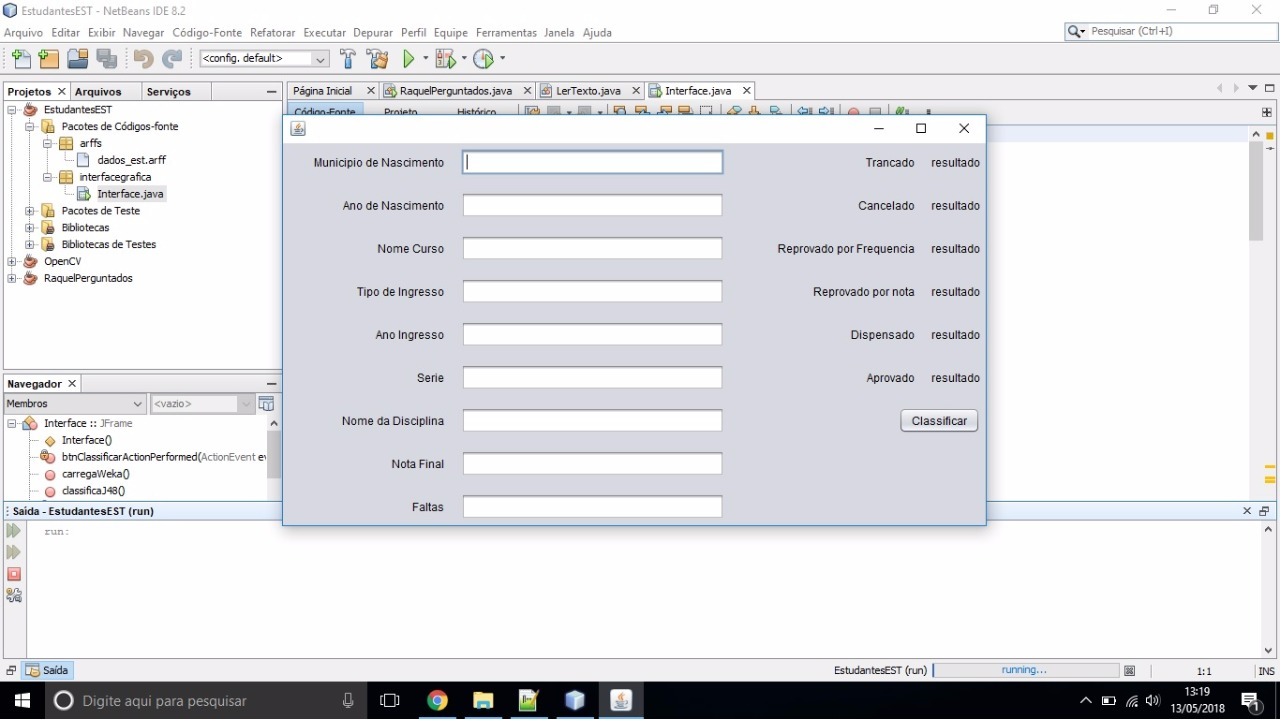
\includegraphics[width=.9\textwidth]{template-latex/sem-dados.jpg}
\caption{Sistema sem os dados}
\label{fig:exampleFig1}
\end{figure}

%---------Figura 2

\begin{figure}[htt]
\centering
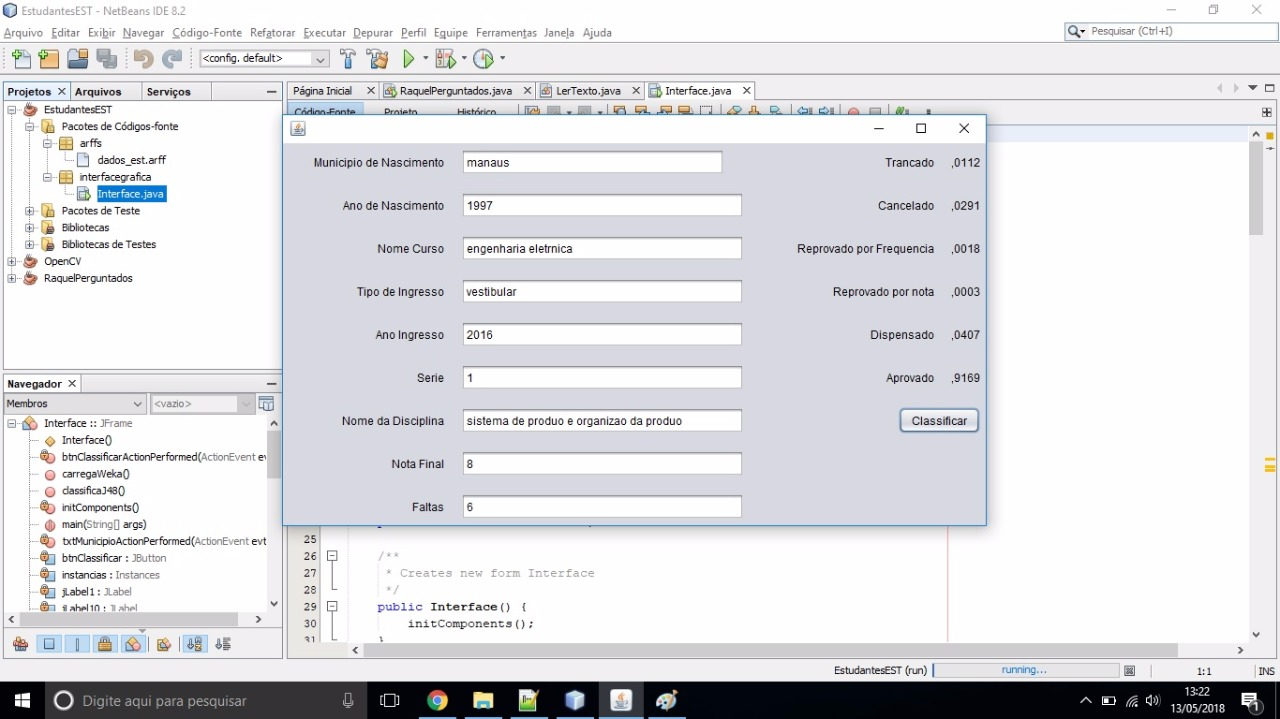
\includegraphics[width=.9\textwidth]{template-latex/com-dados.jpg}
\caption{Sistema com os dados já inseridos}
\label{fig:exampleFig2}
\end{figure}

%----------------------FIM DOCUMENTO = END{BEGIN}
\end{document}
